\section{Présentation}

Il s'agit d'une UE très exigeante sur la maîtrise d'un noyau et d'oeuvres avancées
du C.\\
L'objectif de l'UE est de maîtriser à terme le développement au sein d'un Noyau
Linux, le déboguage avec des outils adaptés et la programmation par patch et
modules.

\begin{itemize}
  \item Examen final : 40\%
  \item Projet \& Exercices : 60\%
\end{itemize}

Deux choses à noter :
\begin{itemize}
  \item Ce cours serait un très obn cours de génie logiciel : plusieurs milliers de
contributeurs, un code très stable et viable car codé de manière très codifiée.
  \item Même sans développer dans le noyau Linux plus tard : il est important de
connaître et de comprendre le système d'exploitation et les outils \& bonnes
pratiques.
\end{itemize}

\subsection{L'origine de "Unix"}
Le nom UNIX fait réference au syst\`eme d'exploitation MULTICS (MULTiplexed
Information and Computing System) issu d'une collaboration entre le MIT, Bell
\& General Electric.
Plusieurs rumeurs tounre autour de l'origine du mot.\\

\section{Systèmes d'Exploitation - Rappels}
Qu'est ce qu'un système d'exploitation, en essence? $\Rightarrow$ Un gestionnaire
d'interruption.
Il y a quatres types de Noyau:

\subsection{Noyaux monolithiques}
\begin{center}
  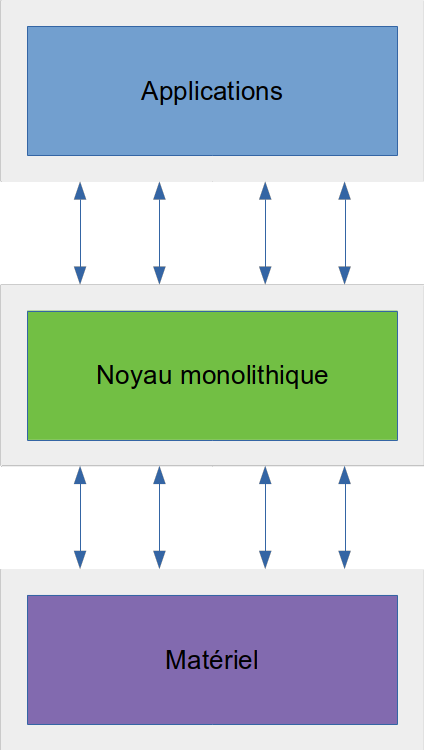
\includegraphics[height=10cm]{cours1/pics/cours1_monolith.png}
\end{center}
Un noyau compilé statiquement, sur un seul binaire (UNICSV6 par exemple).
\\
WARN : un noyau monolithique ne veut pas dire un code monolithique
Le noyau fournit aux applications utilisateurs une abstraction concernant les
abstractions du matériel. Communiquer de l'application au matériel se passe par
le biais d'interruptions $\Rightarrow$ mapper différentes interruptions à différentes
actions.

Un OS se distingue par deux modes d'exécution différents : le mode système et le
mode utilisateur. Le premier possède des avantages tels que :
\begin{itemize}
  \item Zones mémoire restreintes
  \item Instructions privilégiées
  \item Pile spécifique
  \item Accès à certains registres
\end{itemize}

Intérêts :
\begin{itemize}
  \item Facile à optimiser car sur la même codebase $\Rightarrow$ performant
  \item Facile à sécuriser
\end{itemize}
Inconvénients :
\begin{itemize}
  \item Empreinte mémoire assez importante quand non-dédiée
  \item Beaucoup de fonctionnalités $\Rightarrow$ Beaucoup de failles potentielles
\end{itemize}

Utilisation du noyau monolithique $\Rightarrow$ embarqué, applications RT ou
spécifique.

\subsection{Micro-noyaux}

\begin{center}
  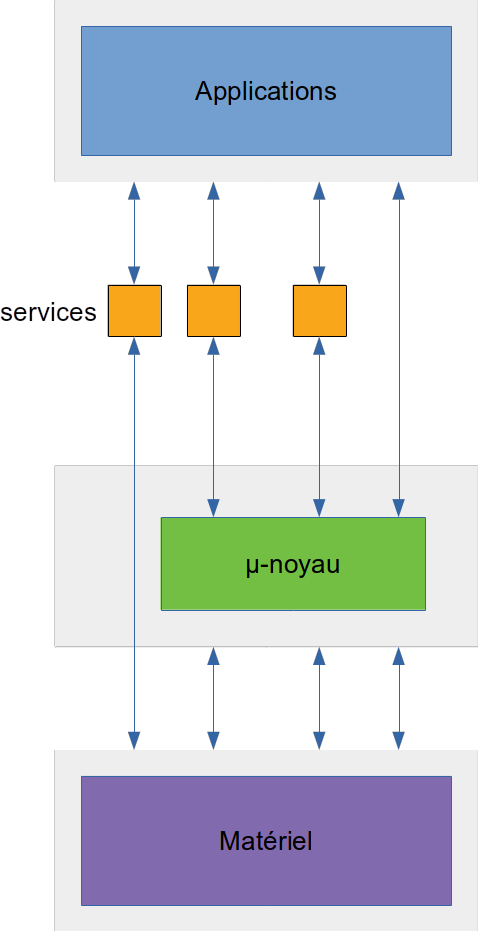
\includegraphics[height=10cm]{cours1/pics/cours1_micro.png}
\end{center}
Idée : Réduire le noyau à un set de fonctionnalités fondamentales, et mettre les
autres services en mode utilisateurs. On réduit la surface d'attaque du
noyau en dispatchant dans le mode utilisateur (exemple : filesystems)\\\\
Intérêts :
\begin{itemize}
  \item Empreinte mémoire très réduite
  \item Surface d'attaque très restreinte
  \item Fonctionnalités en mode utilisateur $\Rightarrow$ execution en mode utilisateur
\end{itemize}
Inconvénients :
\begin{itemize}
  \item Beaucoup d'appels systèmes $\Rightarrow$ impact sur les performances
  \item Codebase dispatchée $\Rightarrow$ plus difficile à tenir à jour
\end{itemize}
\subsection{Noyaux modulaires monolithiques}
\begin{center}
  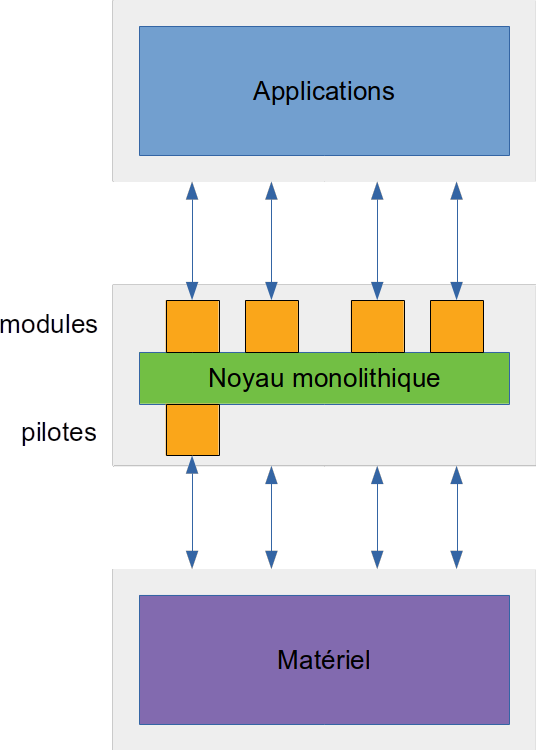
\includegraphics[height=10cm]{cours1/pics/cours1_monolithmod.png}
\end{center}
Avoir un noyau monolithique auquel on peut charger des modules.
Intérêts :
\begin{itemize}
  \item Interaction directe avec le matériel optimisé
  \item Possibilité d'opti pour une architecture
  \item facile d'extension et de portabilité
  \item Modules directement en mode privilégié
\end{itemize}
Inconvénients :
\begin{itemize}
  \item Pas très portable
  \item Modules tiers en mode privilégié $\Rightarrow$ sécurité compromise!
\end{itemize}
Nb : il est possible de hard link des modules pour faire de la programmation
monolithique.
\subsection{Micro-noyaux modulaires}
\begin{center}
  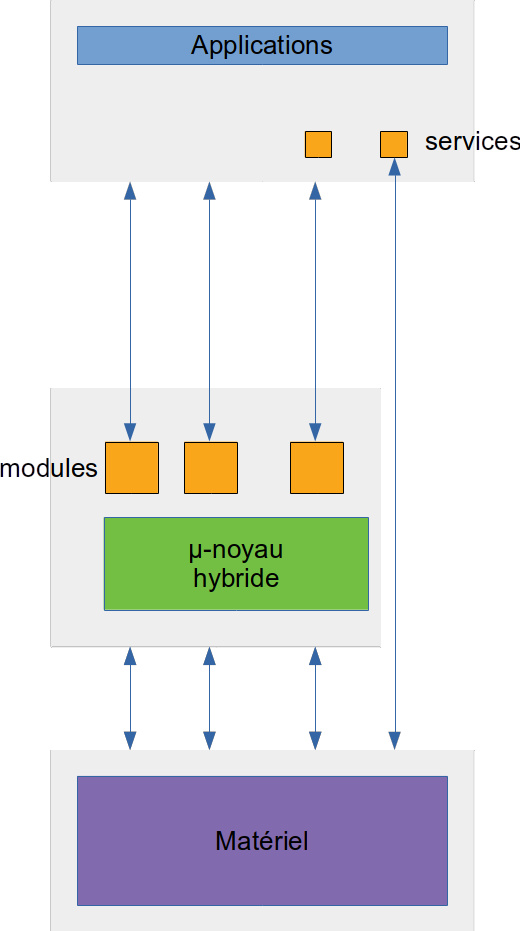
\includegraphics[height=10cm]{cours1/pics/cours1_micromod.png}
  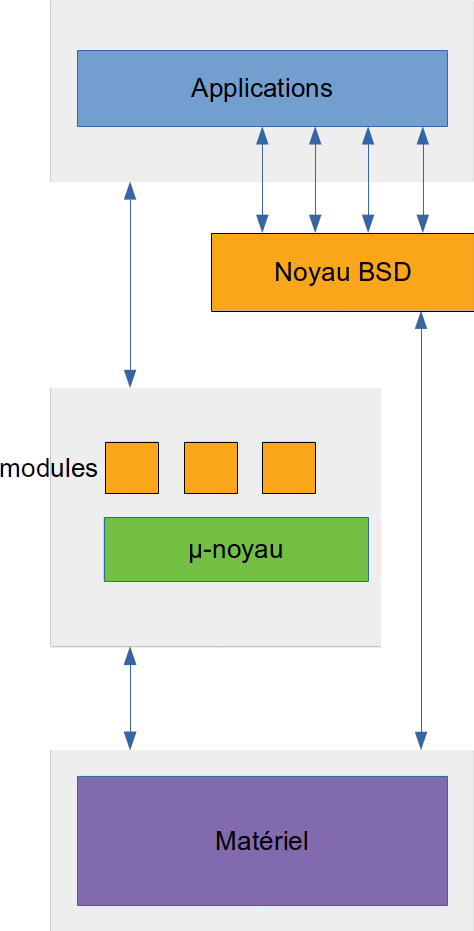
\includegraphics[height=10cm]{cours1/pics/cours1_mach.png}
\end{center}
Possibilité d'avoir d'une part des services haut-niveau opérés en mode utilisateur
et un micro-noyau modulaire. Cela permet de combiner les avantages de modularités
des micro-noyaux et des noyaux monolithiques modulaires.

On pourrait dire que parce que glibc est l'API de choix des développeurs sous
Linux, Linux est quelque part un micro-noyau modulaire.

Pourquoi BSD : problème de licence. Si on utlisait GNU Linux, il y aurait
obligation de laisser les codes sources sous GNU libres.
\subsection{Exo-noyau}
\begin{center}
  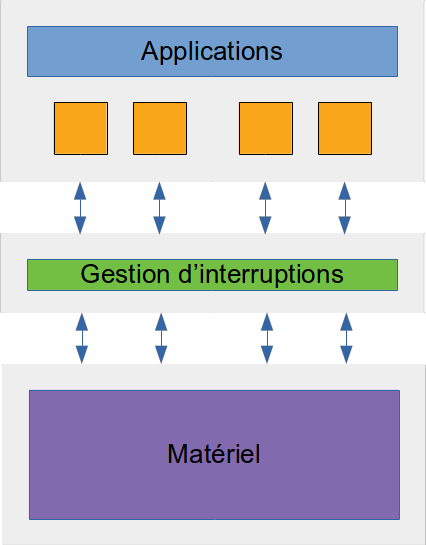
\includegraphics[height=10cm]{cours1/pics/cours1_exo.png}
\end{center}
Le noyau est réduit à l'interception et redirection d'interruptions. Les applications
ont la charge de la gestion de la mémoire et des périphériques.
\subsection{Uni-Kernel}
\begin{center}
  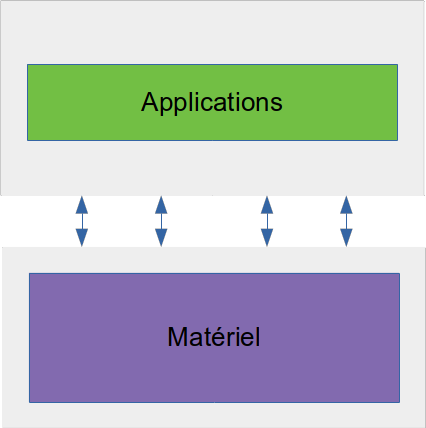
\includegraphics[height=10cm]{cours1/pics/cours1_uni.png}
\end{center}
Une seule application en exécution dans le noyau. En vogue dans le domaine des
syst\`emes embarqu\'es. Ces uni-kernels sont ensuite encapsul\'ees en VM, et
chaqu'une possédant son propre espace mémoire.
